% $Header: /home/vedranm/bitbucket/beamer/solutions/conference-talks/conference-ornate-20min.en.tex,v 90e850259b8b 2007/01/28 20:48:30 tantau $

\documentclass{beamer}

% This file is a solution template for:

% - Talk at a conference/colloquium.
% - Talk length is about 20min.
% - Style is ornate.



% Copyright 2004 by Till Tantau <tantau@users.sourceforge.net>.
%
% In principle, this file can be redistributed and/or modified under
% the terms of the GNU Public License, version 2.
%
% However, this file is supposed to be a template to be modified
% for your own needs. For this reason, if you use this file as a
% template and not specifically distribute it as part of a another
% package/program, I grant the extra permission to freely copy and
% modify this file as you see fit and even to delete this copyright
% notice. 


\mode<presentation>
{
  \usetheme{Warsaw}
  % or ...

  \setbeamercovered{transparent}
  % or whatever (possibly just delete it)
}


\usepackage[english]{babel}
% or whatever

\usepackage[latin1]{inputenc}
% or whatever

\usepackage{times}
\usepackage[T1]{fontenc}
% Or whatever. Note that the encoding and the font should match. If T1
% does not look nice, try deleting the line with the fontenc.
\usepackage{graphicx}

\title{Semi-automated point cloud cleaning}

\author{Rickert Mulder}
% - Give the names in the same order as the appear in the paper.
% - Use the \inst{?} command only if the authors have different
%   affiliation.

\institute[U of X]
{
  Department of Computer Science\\
  University of Cape Town
}

\date[CFP 2003] % (optional, should be abbreviation of conference name)
{Masters Proposal}
% - Either use conference name or its abbreviation.
% - Not really informative to the audience, more for people (including
%   yourself) who are reading the slides online

\subject{Computer Science}
% This is only inserted into the PDF information catalog. Can be left
% out. 



% If you have a file called "university-logo-filename.xxx", where xxx
% is a graphic format that can be processed by latex or pdflatex,
% resp., then you can add a logo as follows:

% \pgfdeclareimage[height=0.5cm]{university-logo}{university-logo-filename}
% \logo{\pgfuseimage{university-logo}}



% Delete this, if you do not want the table of contents to pop up at
% the beginning of each subsection:
\AtBeginSubsection[]
{
  \begin{frame}<beamer>{Outline}
    \tableofcontents[currentsection,currentsubsection]
  \end{frame}
}


% If you wish to uncover everything in a step-wise fashion, uncomment
% the following command: 

%\beamerdefaultoverlayspecification{<+->}


\begin{document}

\begin{frame}
  \titlepage
\end{frame}

\begin{frame}{Outline}
  \tableofcontents
  % You might wish to add the option [pausesections]
\end{frame}


% Structuring a talk is a difficult task and the following structure
% may not be suitable. Here are some rules that apply for this
% solution: 

% - Exactly two or three sections (other than the summary).
% - At *most* three subsections per section.
% - Talk about 30s to 2min per frame. So there should be between about
%   15 and 30 frames, all told.

% - A conference audience is likely to know very little of what you
%   are going to talk about. So *simplify*!
% - In a 20min talk, getting the main ideas across is hard
%   enough. Leave out details, even if it means being less precise than
%   you think necessary.
% - If you omit details that are vital to the proof/implementation,
%   just say so once. Everybody will be happy with that.

\section{Motivation}

\subsection{Background}

\begin{frame}{The Zamani Project}
  % - A title should summarize the slide in an understandable fashion
  %   for anyone how does not follow everything on the slide itself.

  
\includegraphics[width=0.70\textwidth]{pics/Zamani_logo}

  \begin{itemize}
  \item
    Cultural heritage preservation.
  \item
    Capture the spatial domain of heritage sites.
  \end{itemize}
\end{frame}

\begin{frame}{Capturing the Spatial Domain}
  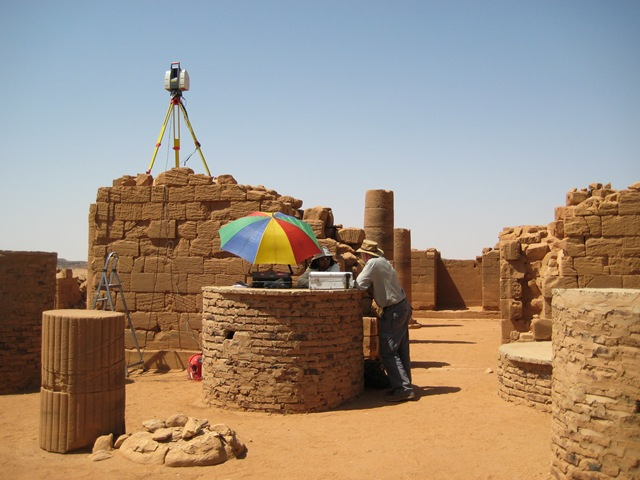
\includegraphics[width=0.60\textwidth]{pics/scanning.jpg}
    \begin{itemize}
  \item
    Laser range scanning.
  \item
    Site photography.
  \end{itemize}
\end{frame}

\begin{frame}{Processing Pipeline}
  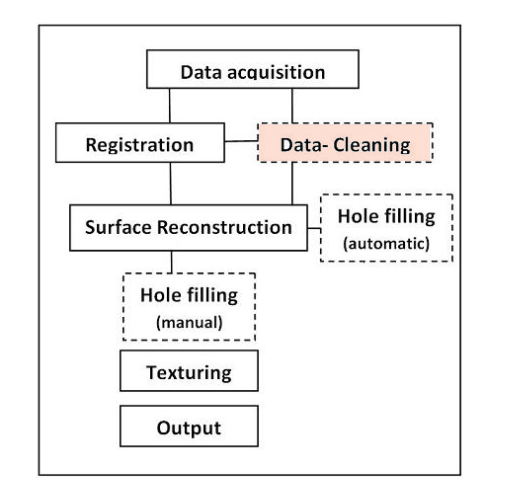
\includegraphics[width=0.50\textwidth]{pics/pipeline.png}
  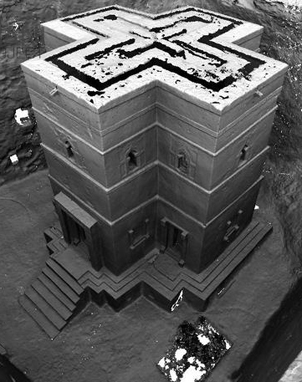
\includegraphics[width=0.38\textwidth]{pics/zamani2.jpg}
\end{frame}

\begin{frame}{Cleaning}
  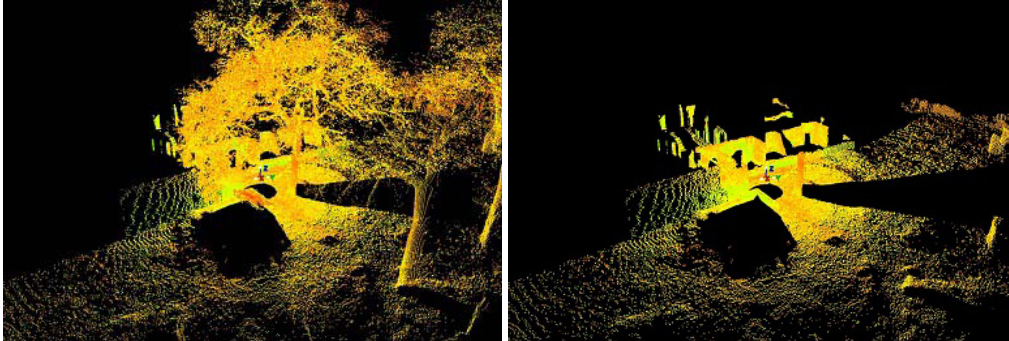
\includegraphics[width=1\textwidth]{pics/cleaning.png}
  \begin{itemize}
  \item
  Cleaning is the removal of unwanted objects
  \item
  It can happen before or after registration.
  % duplication of work
  % more memory requirements
  % size of data input should be noted
  \end{itemize}
\end{frame}

\begin{frame}{Problem}
  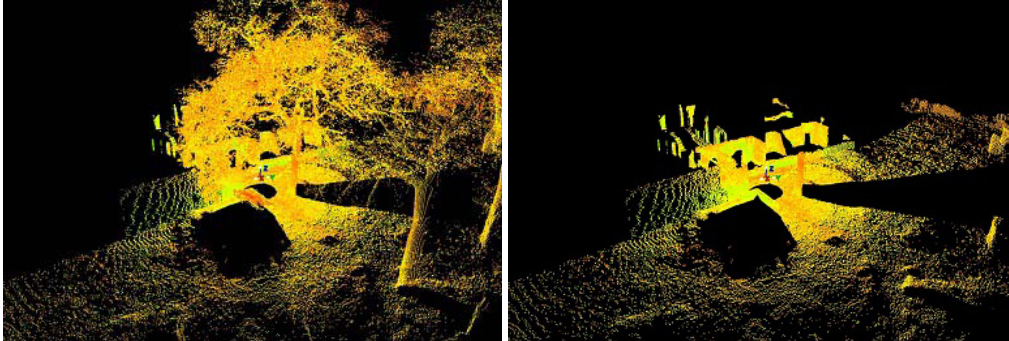
\includegraphics[width=1\textwidth]{pics/cleaning.png}
  \begin{itemize}
  \item
  Cleaning is a manual task
  \item
  500 - 1000 scans per expedition
  \item
  30 min to 2 hours per scan
  % duplication of work
  % more memory requirements
  % size of data input should be noted
  \end{itemize}
\end{frame}

\subsection{Previous Work}

\begin{frame}{Make Titles Informative.}

\begin{figure}[htb]
\centering
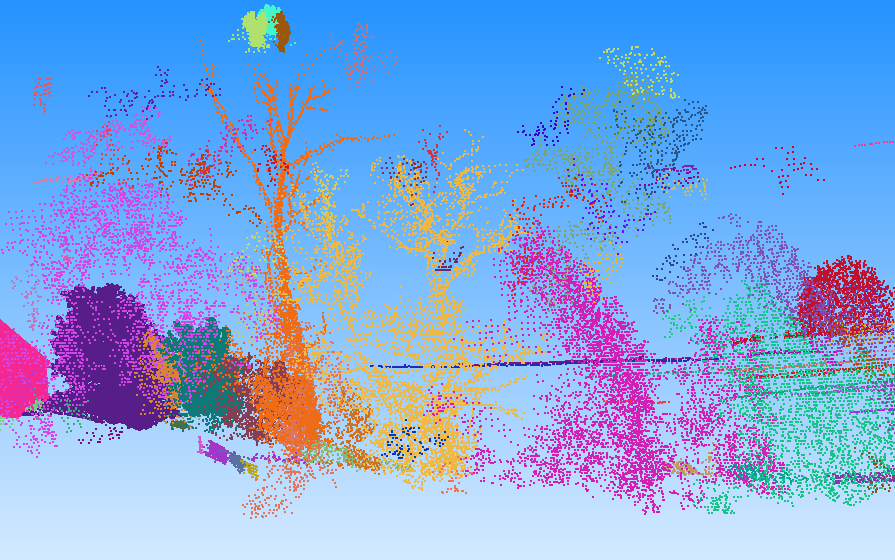
\includegraphics[width=0.70\textwidth]{pics/3dreshaper.png}
\caption{Distance clustering \cite{Technodigit2012}}
\label{fig:dist}
\end{figure}

\end{frame}
\begin{frame}{Make Titles Informative.}

\begin{figure}[htb]
\centering

\includegraphics[width=0.70\textwidth]{pics/vrmesh.png}
\caption{Automated segmentation of vegetation \cite{VirtualGrid2012}}
\label{fig:trees}
\end{figure}




\end{frame}



\section{Proposal}

\subsection{Technology}

\begin{frame}{Make Titles Informative.}

  
\includegraphics[width=0.33\textwidth]{pics/opengl.png}
  
\includegraphics[width=0.33\textwidth]{pics/opencl.png}
  
\includegraphics[width=0.33\textwidth]{pics/pointcloudlibrary_vert_large_pos.png}

\end{frame}

\begin{frame}{Make Titles Informative.}
\end{frame}

\begin{frame}{Make Titles Informative.}
\end{frame}


\subsection{Basic Ideas for Proofs/Implementation}

\begin{frame}{Make Titles Informative.}
\end{frame}

\begin{frame}{Make Titles Informative.}
\end{frame}

\begin{frame}{Make Titles Informative.}
\end{frame}



\section*{Summary}

\begin{frame}{Summary}

  % Keep the summary *very short*.
  \begin{itemize}
  \item
    The \alert{first main message} of your talk in one or two lines.
  \item
    The \alert{second main message} of your talk in one or two lines.
  \item
    Perhaps a \alert{third message}, but not more than that.
  \end{itemize}
  
  % The following outlook is optional.
  \vskip0pt plus.5fill
  \begin{itemize}
  \item
    Outlook
    \begin{itemize}
    \item
      Something you haven't solved.
    \item
      Something else you haven't solved.
    \end{itemize}
  \end{itemize}
\end{frame}



% All of the following is optional and typically not needed. 
\appendix
\section<presentation>*{\appendixname}
\subsection<presentation>*{For Further Reading}

\begin{frame}[allowframebreaks]
  \frametitle<presentation>{For Further Reading}
    
  \begin{thebibliography}{10}
    
  \beamertemplatebookbibitems
  % Start with overview books.

  \bibitem{Author1990}
    A.~Author.
    \newblock {\em Handbook of Everything}.
    \newblock Some Press, 1990.
 
    
  \beamertemplatearticlebibitems
  % Followed by interesting articles. Keep the list short. 

  \bibitem{Someone2000}
    S.~Someone.
    \newblock On this and that.
    \newblock {\em Journal of This and That}, 2(1):50--100,
    2000.
  \end{thebibliography}
\end{frame}

\end{document}


